\chapter{B+ Tree Implementations}\label{chapter:b-tree_implementations}
\section{B+ Tree}
\subsection{Structure}
The original paper on B-Trees \parencite{ogbtree} describes a data structure, where data is managed in a tree-like structure, with a node containing data, and having children with one node being on top, called the root. According to Graefe \parencite{modernbtree} it has self-balanced mechanisms that ensure that the data is remained sorted and lookups require an efficient amount of comparisons by the utilizing binary sort techniques. In Figure \ref{fig:btreeexample} the root node contains three values and references the children in a sorted manner.
\begin{figure}[h]
  \centering
  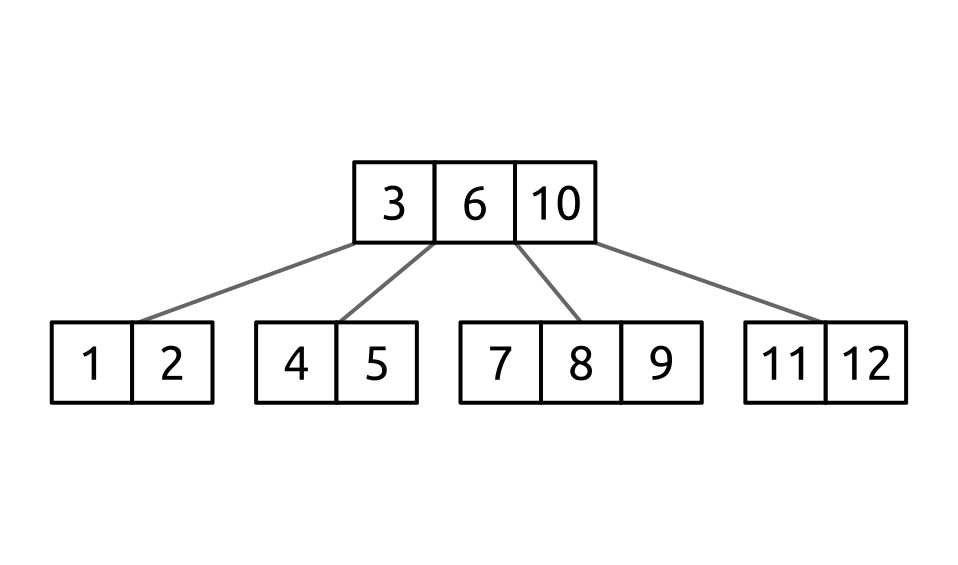
\includegraphics[width=0.5\textwidth]{images/an-example-b-tree.png}
  \caption{Simple B-Tree example \parencite{btreeexample}}
  \label{fig:btreeexample}
\end{figure}
\\\\
Graefe \parencite{modernbtree} further discusses that B+ tree is a variant of the B-tree. Instead of storing the values inside the all nodes it stores the values in the lowest layer, called the leaf nodes. The inner nodes keep track of the keys and reference child nodes, in a sorted manner. To be able to traverse key ranges fast, the leaf nodes can contain a reference to the neighboring leaf node. The implementation by Müller et al. \parencite{mueller2024} does not implement these references. The figure \ref{fig:b+treeexample} outlines a simple example of this variation. The data is structured by keys and values. For example, the number $3$ represents the key $3$ and the middle leaf node contains the reference to the corresponding value $d_3$. In this figure, the references to neighboring leaf nodes are visualized in dark red.


\begin{figure}[h]
  \centering
  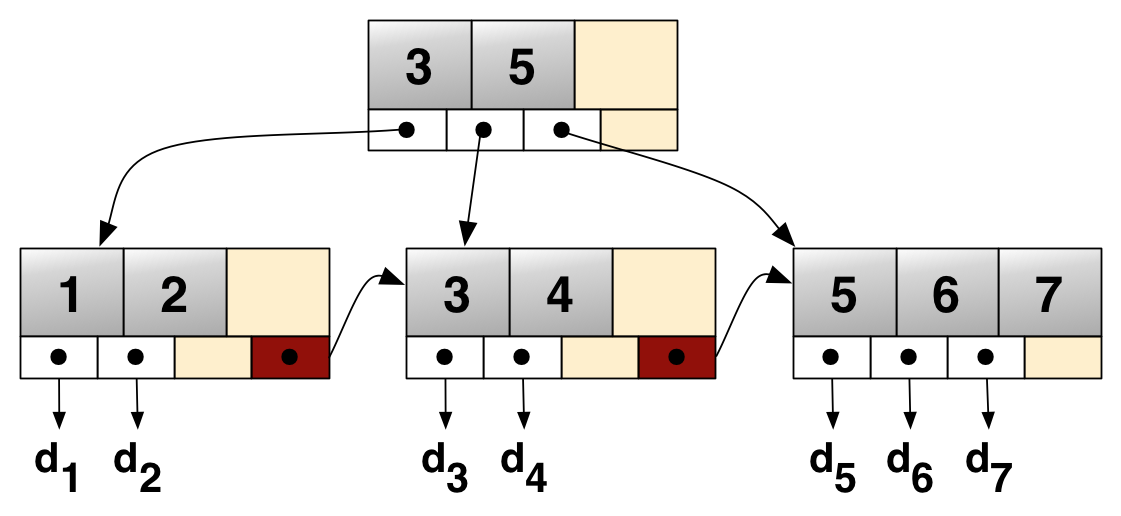
\includegraphics[width=0.5\textwidth]{images/Bplustree.png}
  \caption{Simple B+ tree example \parencite{wikib+tree}}
  \label{fig:b+treeexample}
\end{figure}
 
\subsection{Operations}
The B+ tree, similarly to the B-tree, has, among others, the following operations: Insertion, Search, Deletion, and Range Queries. The differences between the B+ tree and the B-tree lie in the nature of the structures, and therefore the operations have differences in memory usage and performance. Some operations are more suited in a B+ tree than a B-tree. The table \ref{fig:operationstable} outlines the differences in regard to the operations. Overall, a notable downside of B+ trees is the generally bigger storage use, since a B-tree is able to store values in the inner nodes. Graefe \parencite{modernbtree} reported that this downside, however, simplifies some operations, bringing an overall, better performance, making the B+ tree the default structure in modern times. This thesis focuses on the B+ tree and the operations of insertion and range querying. 
\\\\
In this thesis, we consider the operations described in by Müller et al. \parencite{mueller2024}, namely \textbf{insert, remove, lookup, scan} and more specifically the \textbf{insert}, \textbf{lookup} and \textbf{scan} operations.

\begin{table}[htbp]
\centering

\begin{tabular}{|p{2cm}|p{3cm}|p{4cm}|p{4cm}|}
\hline
\textbf{Operation} & \textbf{Description} & \textbf{B-tree} & \textbf{B+ tree} \\
\hline
Search (\textbf{lookup}) & Finding a given key in the tree. & Binary search through the tree & Same as B-tree. \\
\hline
Insertion (\textbf{insert}) & Adding a key-value pair & Values are also stored in internal nodes. & Keys are stored in internal nodes, Values only in leaf nodes. \\
\hline
Deletion (\textbf{remove}) & Removing a key-value pair & Since values are stored in the internal nodes, merging and redistribution operations are more complex. & Simplified merging and redistribution. \\
\hline
Range Queries (\textbf{scan}) & Retrieving a range of keys or values & Less suitable due to values stored in internal nodes. & More suitable because of leaf nodes containing pointers to their succeeding leaf node, which allows sequential access. \\
\hline
Traversal & Iterating through all keys or values in sorted order. & Follows a dept-first approach. & Reduced complexity, since values are only in linked leaf nodes, only requiring one big range query.  \\
\hline
Splitting Nodes & Full nodes are divided into two nodes. & May redistribute keys and values. & Only internal nodes (keys) are affected. Values are not redistributed.  \\
\hline
Merging Nodes & During deletion, nodes may become too empty. Nodes need to be merged as a consequence. & Keys and values need to be redistributed & Simplified as only keys are affected. \\
\hline
\end{tabular}
\caption{Comparison of Operations in B-trees and B+trees}
\label{fig:operationstable}
\end{table}



\section{Optimizations}

The paper by Müller et al. \parencite{mueller2024} uses an implementation of the B+ tree that is implemented in the programming language C++. The paper outlines certain optimizations and configurations that can be utilized with the aim to improve operation runtime performance. The following optimizations have been proposed: 

\begin{itemize}
  \item \textbf{Prefix Truncation} refers to truncating the prefixes that are shared among keys stores in a node. An example for such truncation is cutting off the prefix "\textit{https://}" in url data. This brings benefits to storage use and the cache is better utilized. The key transfer between nodes requires an extra operation, which adds complexity, however as this operation is rare, the runtime cost is minimal. 
  
  \item \textbf{Heads} is the idea of taking the first 4 bytes of the key, named \textit{head}, and using those for the binary search. This enables better use of the cache. The figure \ref{fig:heads} represents this idea by using the first letter of the keys as heads. On the other hand, the slots with heads would require more bytes to be aligned. The implementation by Müller et al. \parencite{mueller2024} decided on doing unaligned access, since the negative impact is believed to be negligible. \\
  
  \begin{figure}[h]
      \centering
      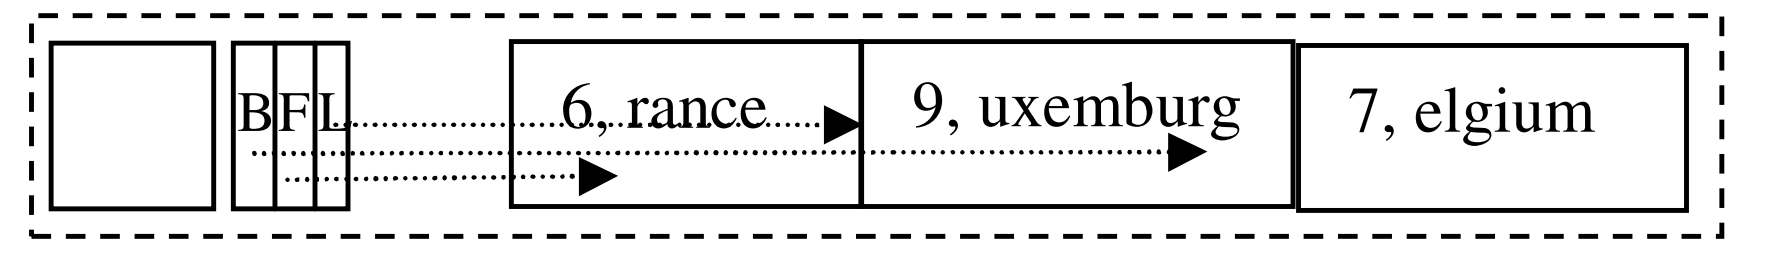
\includegraphics[width=0.5\textwidth]{images/heads.png}
      \caption{Heads example \parencite{modernbtree}}
      \label{fig:heads}
  \end{figure}
    
  \item \textbf{Hints} takes the idea of \textbf{heads} one step further, by adding a structure called hint array to each node header. The array contains the heads of equidistant slots, as visualized in figure \ref{fig:hints}. The implementation by Müller et al. \parencite{mueller2024} sets the hint array to the size of 16 hints, and the array is updated only at or after the insertion. 

  \begin{figure}[h]
      \centering
      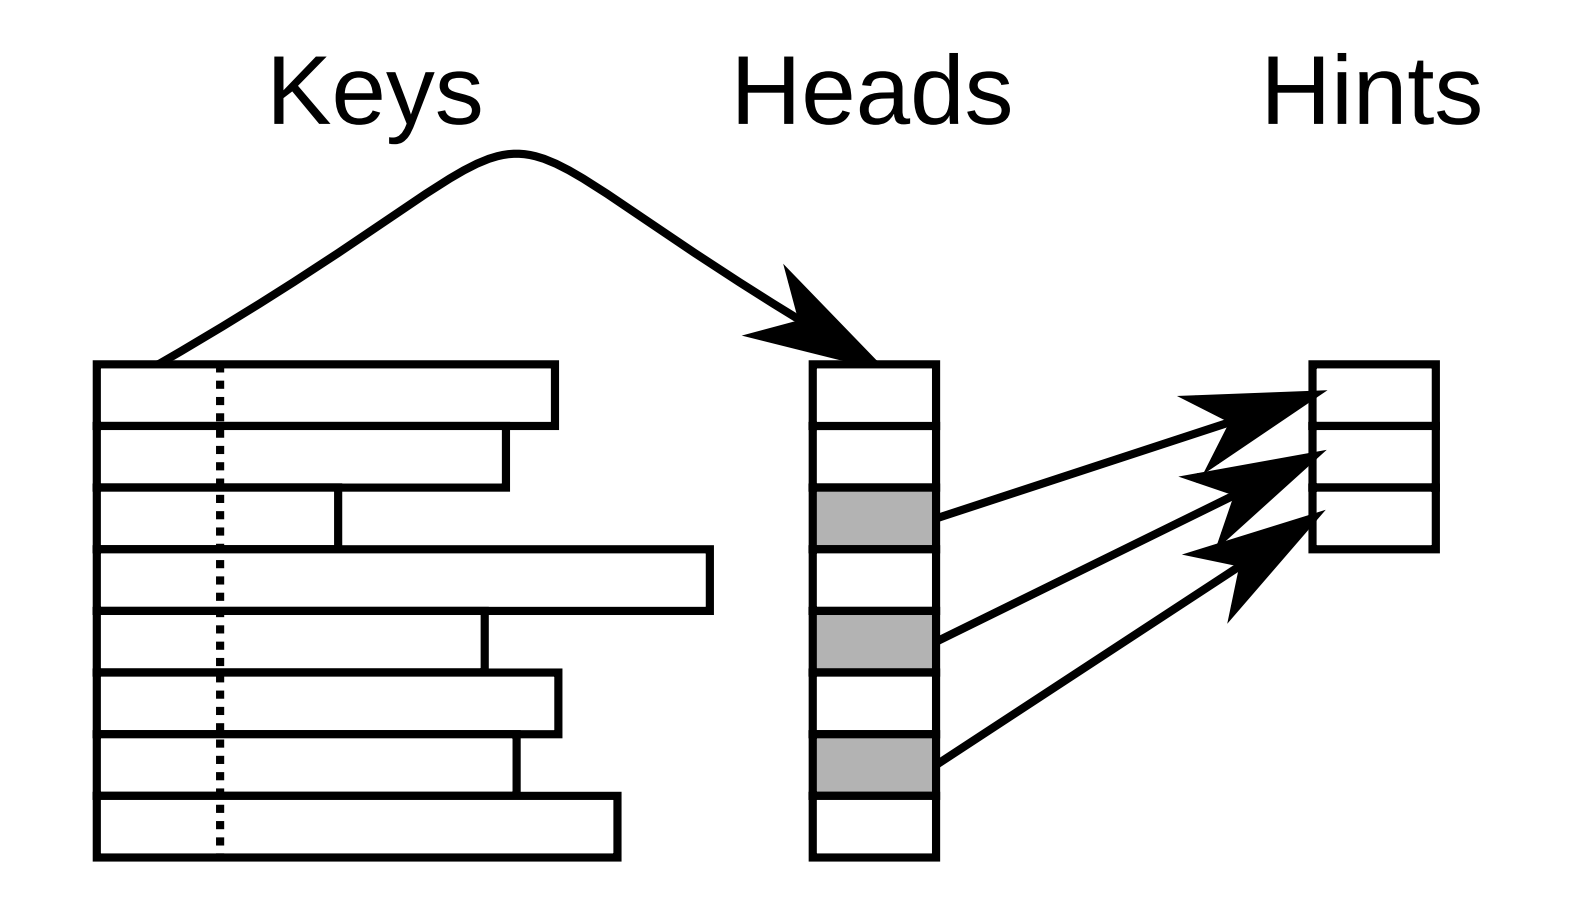
\includegraphics[width=0.5\textwidth]{images/hints.png}
      \caption{Hints from heads \parencite{mueller2024}}
      \label{fig:hints}
  \end{figure}
    
  \item \textbf{Fingerprinting} introduces an array of key hashes in the heap of the node. The figure \ref{fig:hash} is an example for such an array. The array contains a sorted and an unsorted part. During insertion, the values are appended to the end - the unsorted part. The fingerprint array only gets sorting during scan, node splitting, merging operations. If used in combination with \textbf{prefix truncation}, the prefixes get truncated before calculating the hash. Additionally, to improve performance of search operations on nodes the SIMD instructions with a range of 256 bit are used.
  
  \begin{figure}[h]
      \centering
      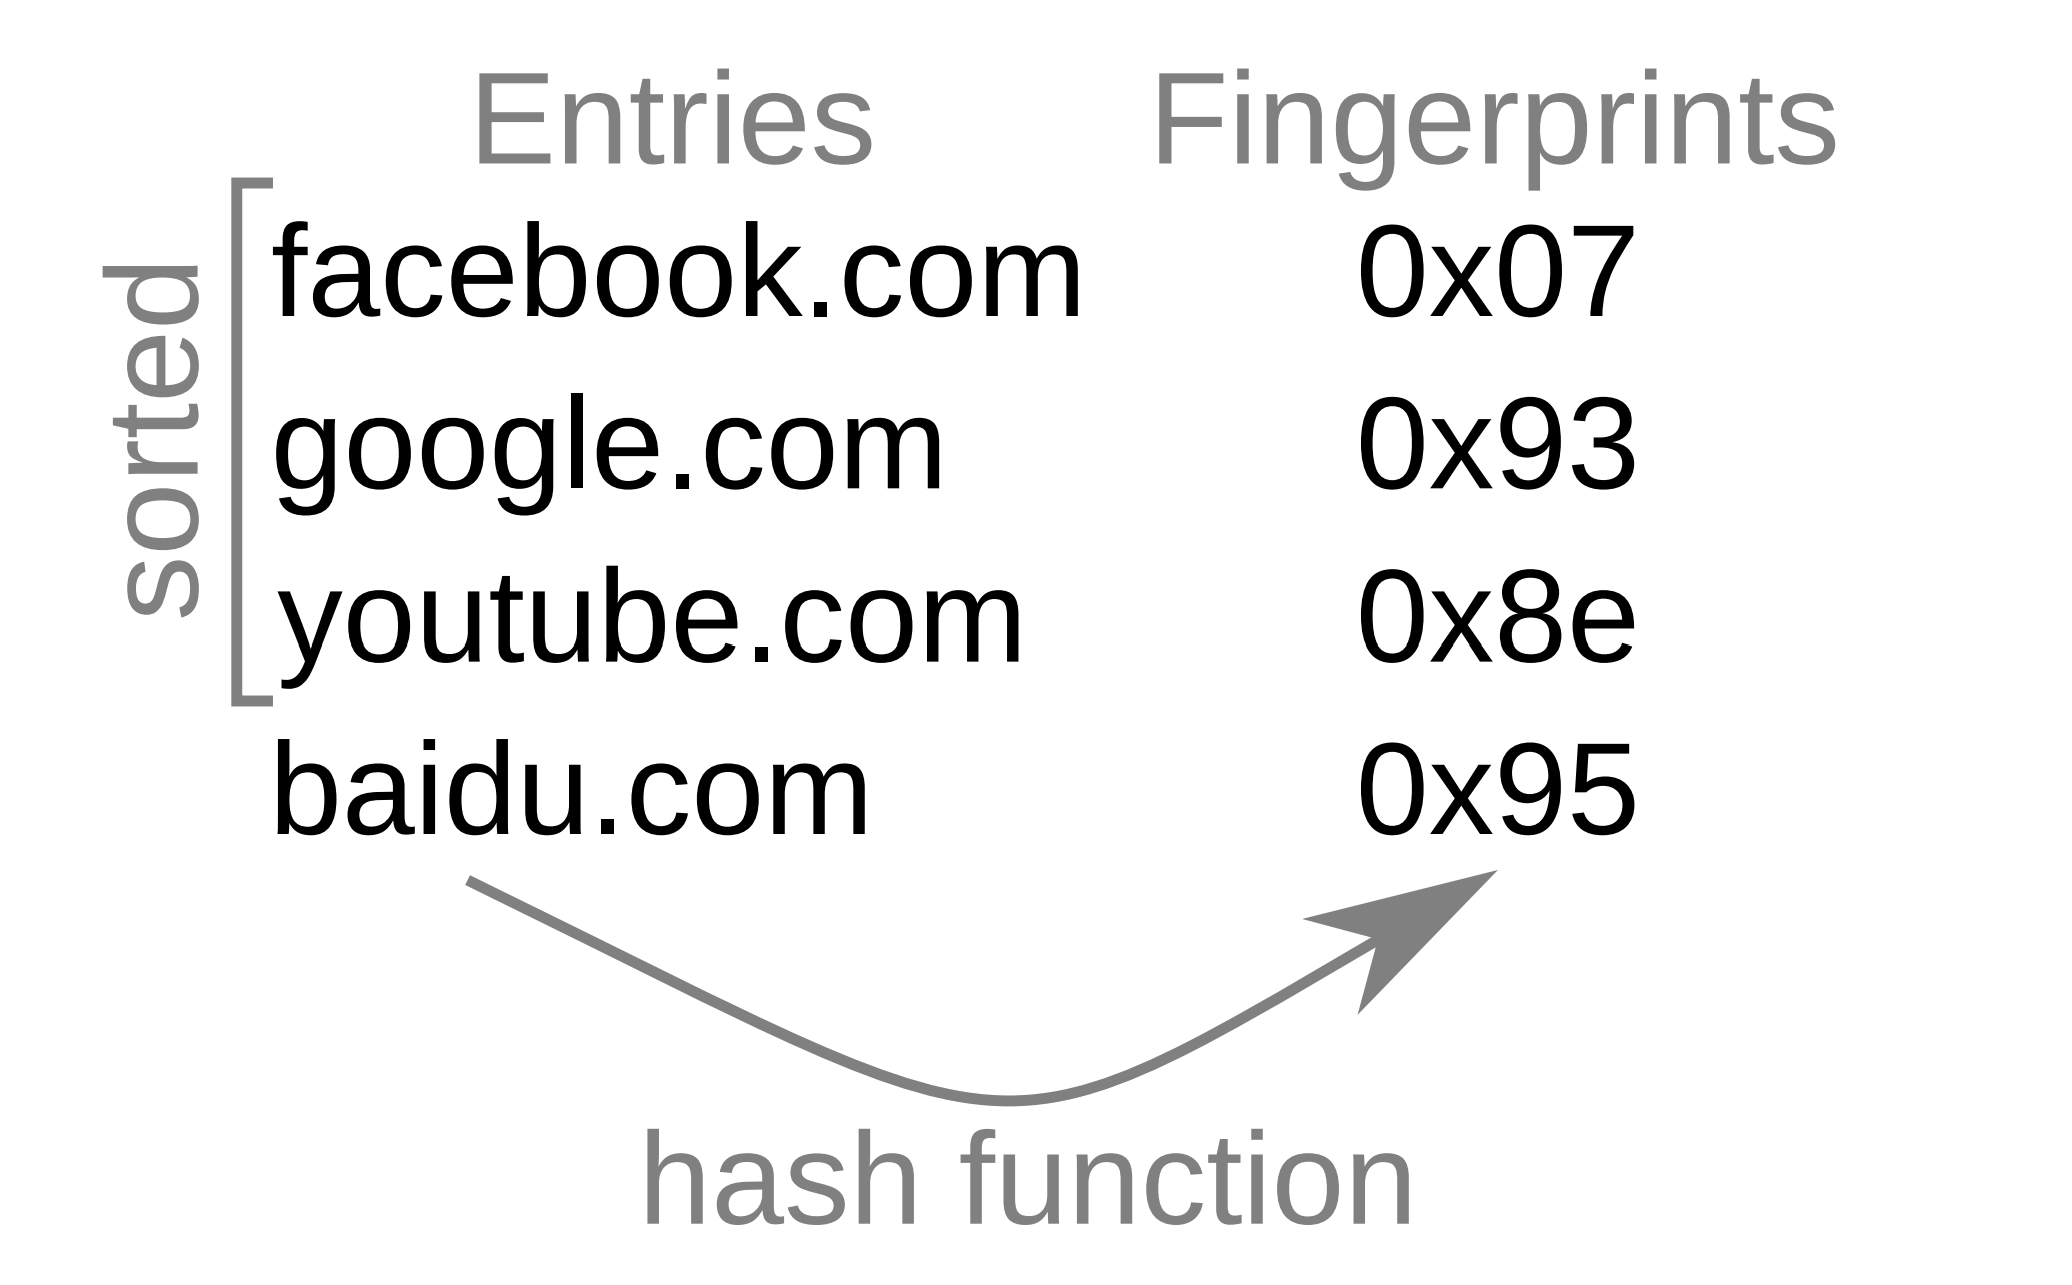
\includegraphics[width=0.5\textwidth]{images/hash.png}
      \caption{Fingerprinting array \parencite{mueller2024}}
      \label{fig:hash}
  \end{figure}
    
  \item \textbf{Dense Leaves} is a new approach introduced by Müller at al. \parencite{mueller2024}, based on the idea of using frame-of-reference encoding to keys. Frame-of-reference encoding takes reference keys and calculates the offsets for the following values. This idea is meant for keys that are dense enough, thereby mitigating the inefficiency associated with underutilized storage space. Two approaches are presented, namely \textbf{Semi Dense Leaves} and \textbf{Fully Dense Leaves}. As presented in figure \ref{fig:denseLeaves}, Semi Dense Leaves contain pointers at each possible offset to the node's heap containing the keys and values. The Fully Dense Leaves implementation presumes that the values are of the same size, which is a common characteristic for specific types of data. Additionally, a partition mechanism is implemented, which recognizes dense keys originating from different sources and therefore ensuring that the tree stores data more densely.

  \begin{figure}[h]
      \centering
      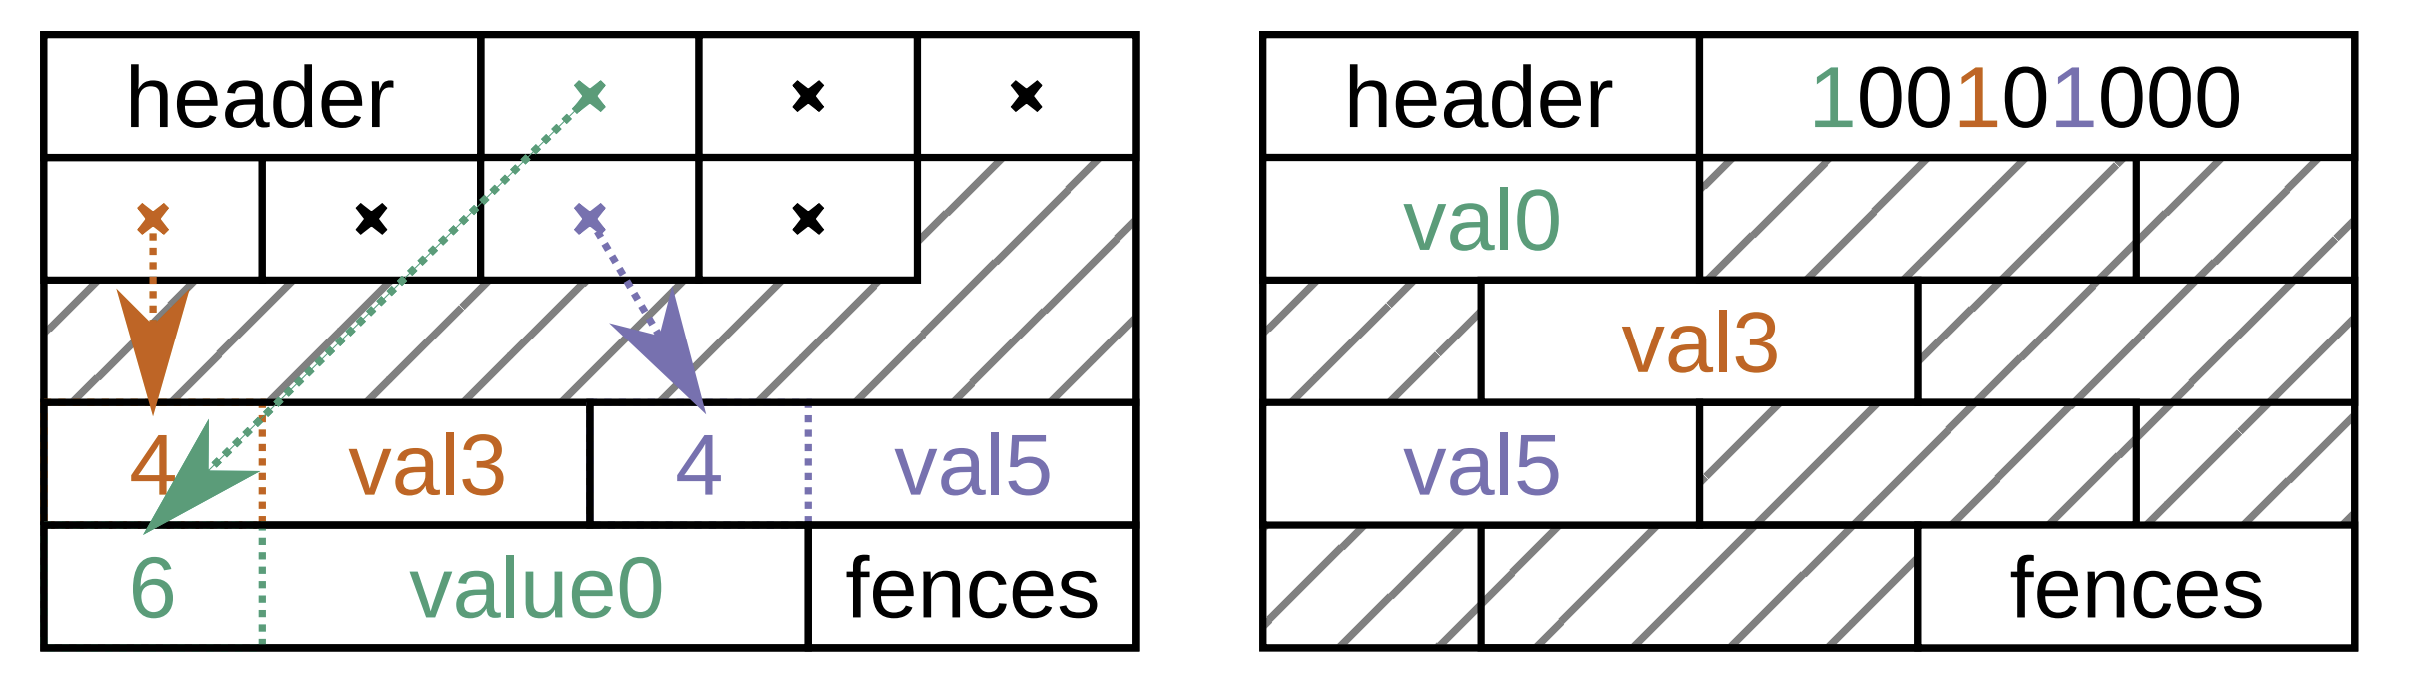
\includegraphics[width=0.5\textwidth]{images/denseLeaves.png}
      \caption{Example of Semi (left) and Fully (right) Dense Leaves with three values \parencite{mueller2024}}
      \label{fig:denseLeaves}
  \end{figure}
     
\end{itemize}

\section{Adaptable B+ tree}
Müller et al. \parencite{mueller2024} further discusses the topic of creating a B+ tree, which is adaptable, meaning that it can adjust the type of leafs to circumstances and the type operations. One approach is proposed, and shows considerable performance improvements in its benchmarks. The figure \ref{fig:adapt} describes, in which circumstances, leafs are transitioned into a different type.
  \begin{figure}[h]
      \centering
      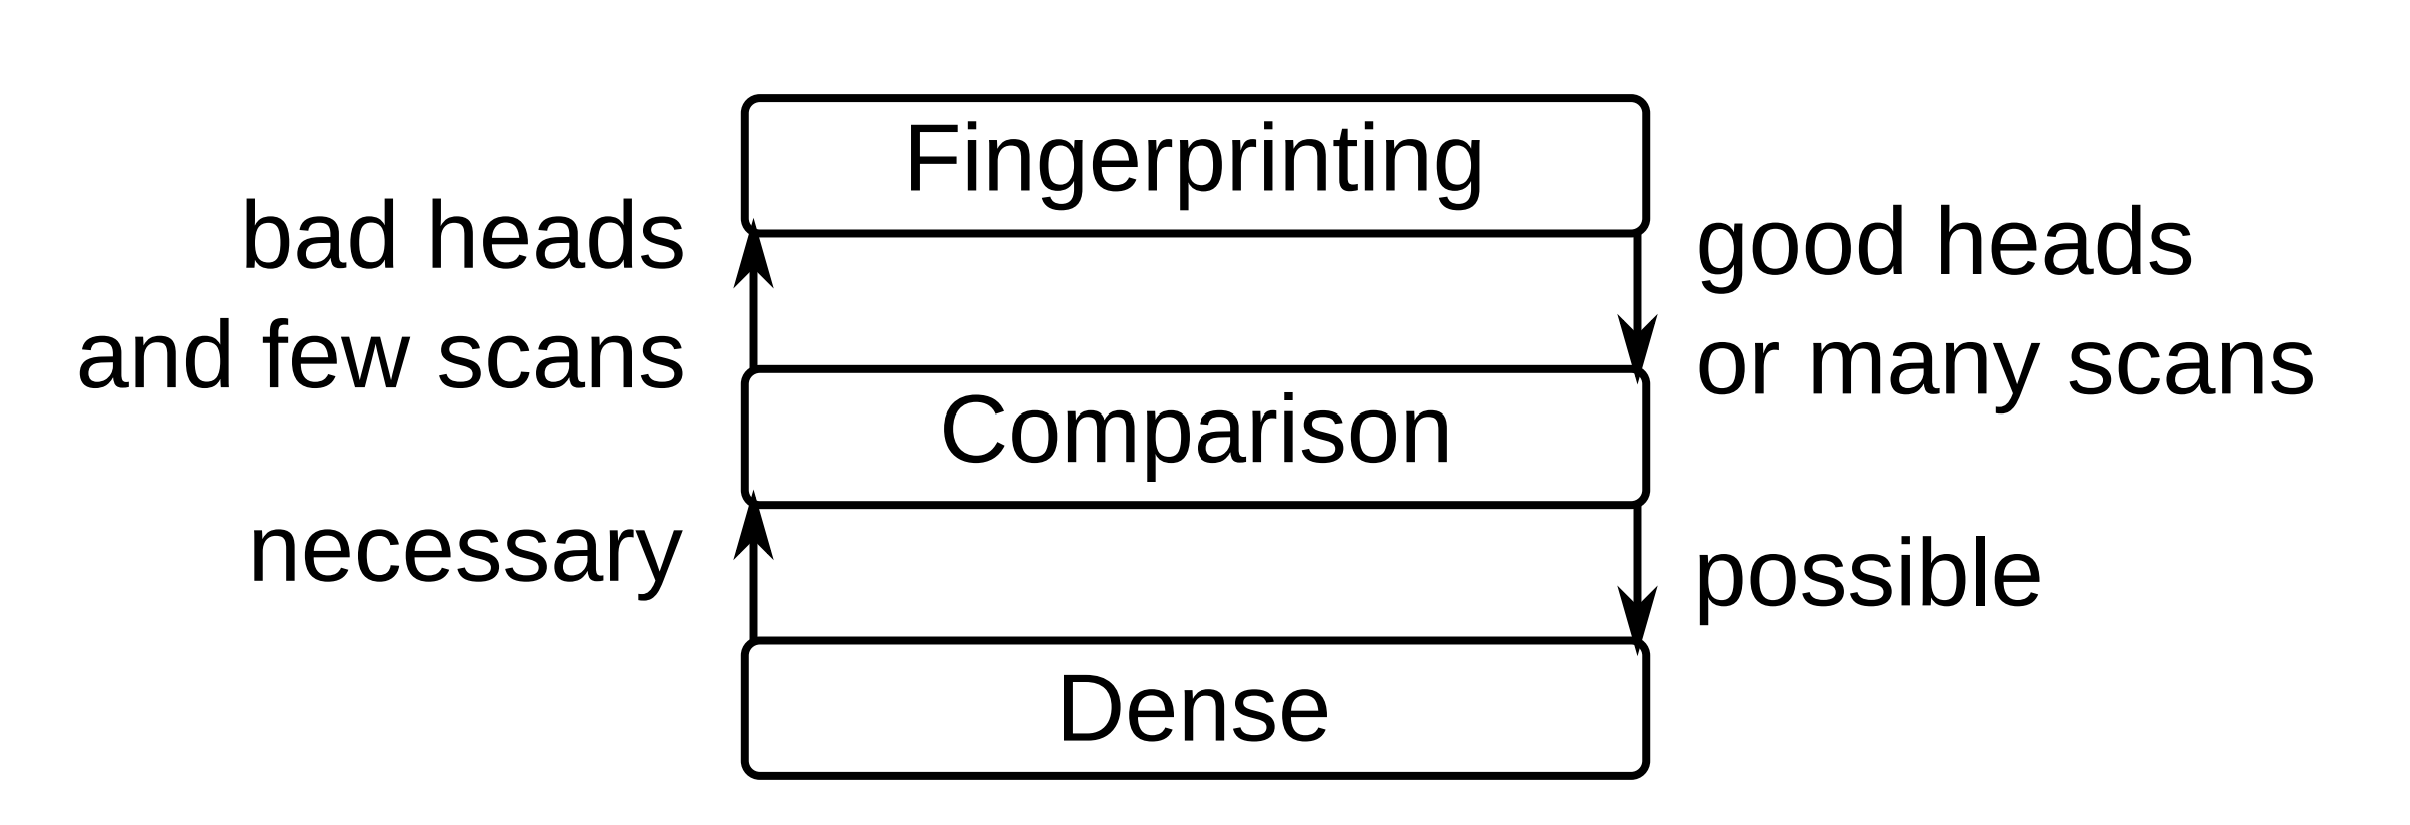
\includegraphics[width=0.5\textwidth]{images/adapt.png}
      \caption{Decisions on leaf layout \parencite{mueller2024}}
      \label{fig:adapt}
  \end{figure}
\\\\
This thesis takes this idea and aims to get more insights into the possible approaches of configuring B+ trees. The goal is to improve on the idea of adaptable B+ trees, by finding factors impacting the performance in various configuration combinations. Particularly, the focus lies on the page size of leaf nodes, since this configuration is easily adaptable during runtime. 